\documentclass[12pt,a4paper]{report}
\usepackage[utf8]{inputenc} % un package
\usepackage[T1]{fontenc} % un second package
\usepackage[francais]{babel} % un troisième package
\usepackage{color} % Package de la couleur
\usepackage{verbatim}
\usepackage{moreverb}
\usepackage{amsmath}
\usepackage{amsfonts}
\usepackage{amssymb}
\usepackage{graphicx}
\usepackage[top=2cm, bottom=2cm, left=2cm, right=2cm]{geometry}
\author{IMA World Health Web Developer Team}
\title{
\includegraphics[width=12cm]{ima.png} \\BASIC HOSPITAL INFORMATION MANAGEMENT APPLICATION\\ (BHIMA) \\ Manuel d'utilisation}

\begin{document}
%Page de garde
\maketitle 
\chapter{Présentation}
\section{Accès au système}
\large{Pour accéder au système, la première de chose à faire est de lancer un navigateur web, en suite saisir l'adresse web de server dans la barre d'adresse du navigateur.}

La première interface de l'application est un formulaire qui demande à chaque utilisateur de pouvoir fournir son login, son mot de passe mais aussi de spécifier  le projet dont il sont assigné, comme le montre le formulaire ci-dessous.
\begin{figure}[h]
\begin{center}
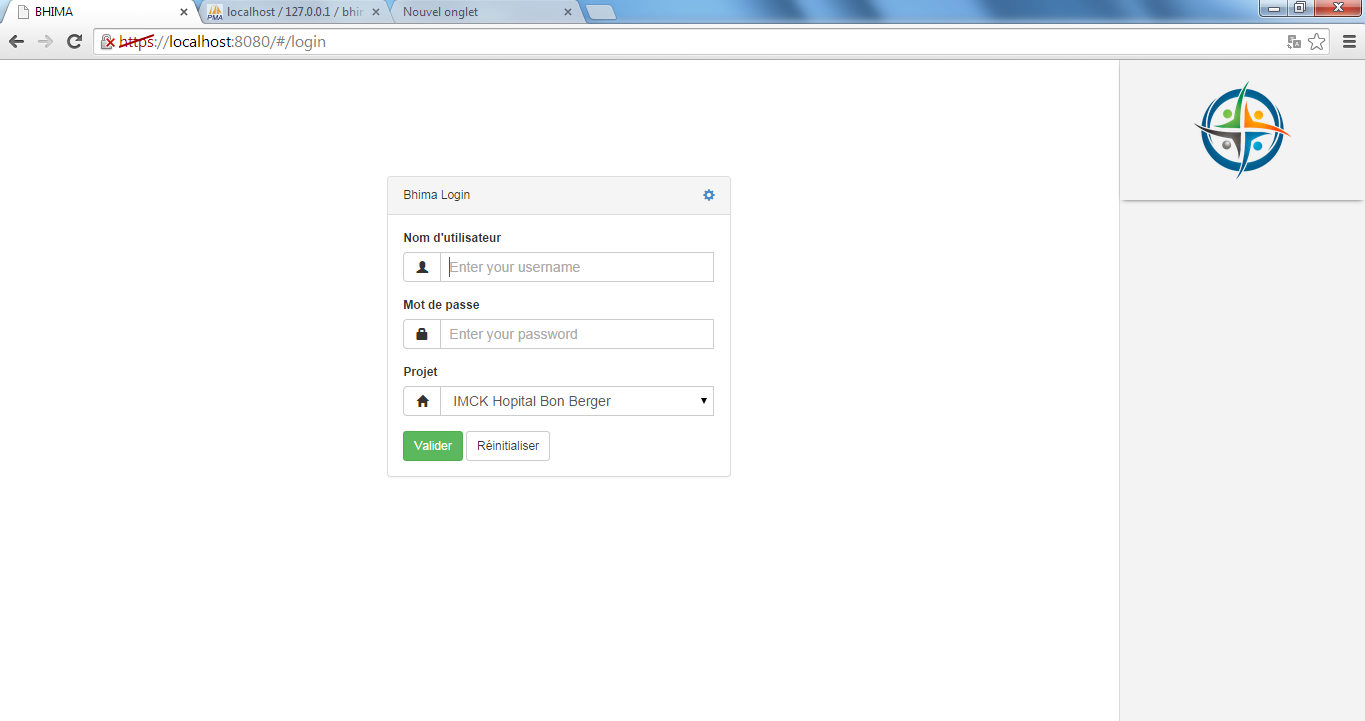
\includegraphics[width=12cm]{pic/login.png}
\end{center}
\caption{Page d'identification et authentification des utilisateurs}
\label{Page d'identification et authentification des utilisateurs}
\end{figure}
\\ L'accès au système n'est garanti que pour ceux qui possèdent un compte utilisateur, si l'utilisateur s'est authentifié alors il sera dirigé vers l'interface principale de l'application qui se présente de la manière suivante.
\newpage
\begin{figure}[h]
\begin{center} 
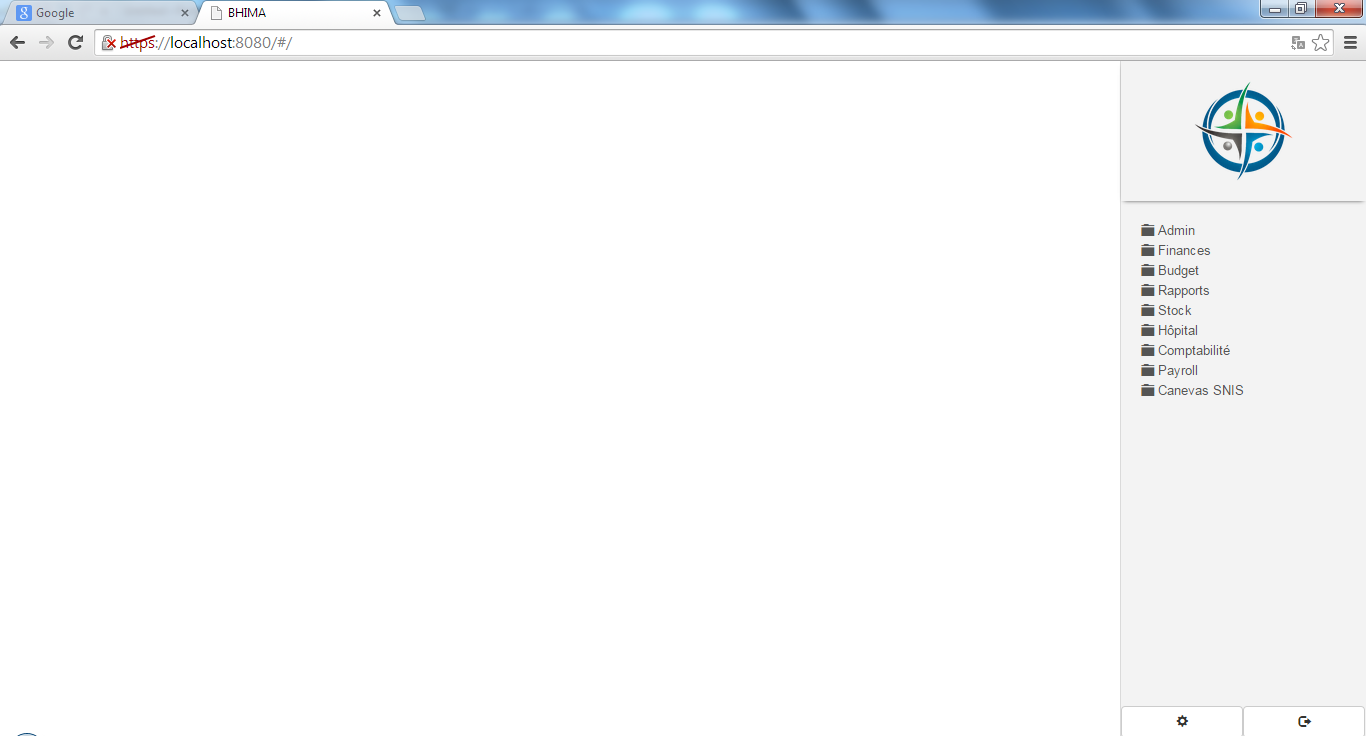
\includegraphics[width=10cm]{pic/mainInterface.png}
\end{center}
\caption{Interface principale de l'application}
\label{Interface principale de l'application}
\end{figure} 
Dans sa partie gauche de la figure ci-dessous on retrouve le logo IMA World Heath Ainsi que l'arborescence qui représente les modules du système auxquels l'utilisateur à accès. En dessous de l'arborescence figure deux boutons, le premier 
\includegraphics[scale=0.5]{pic/lang.png} permet de changer de langue et le second 
\includegraphics[scale=0.5]{pic/logout.png} permet de ce déconnecté du système.

\begin{figure}[h]
\begin{center}
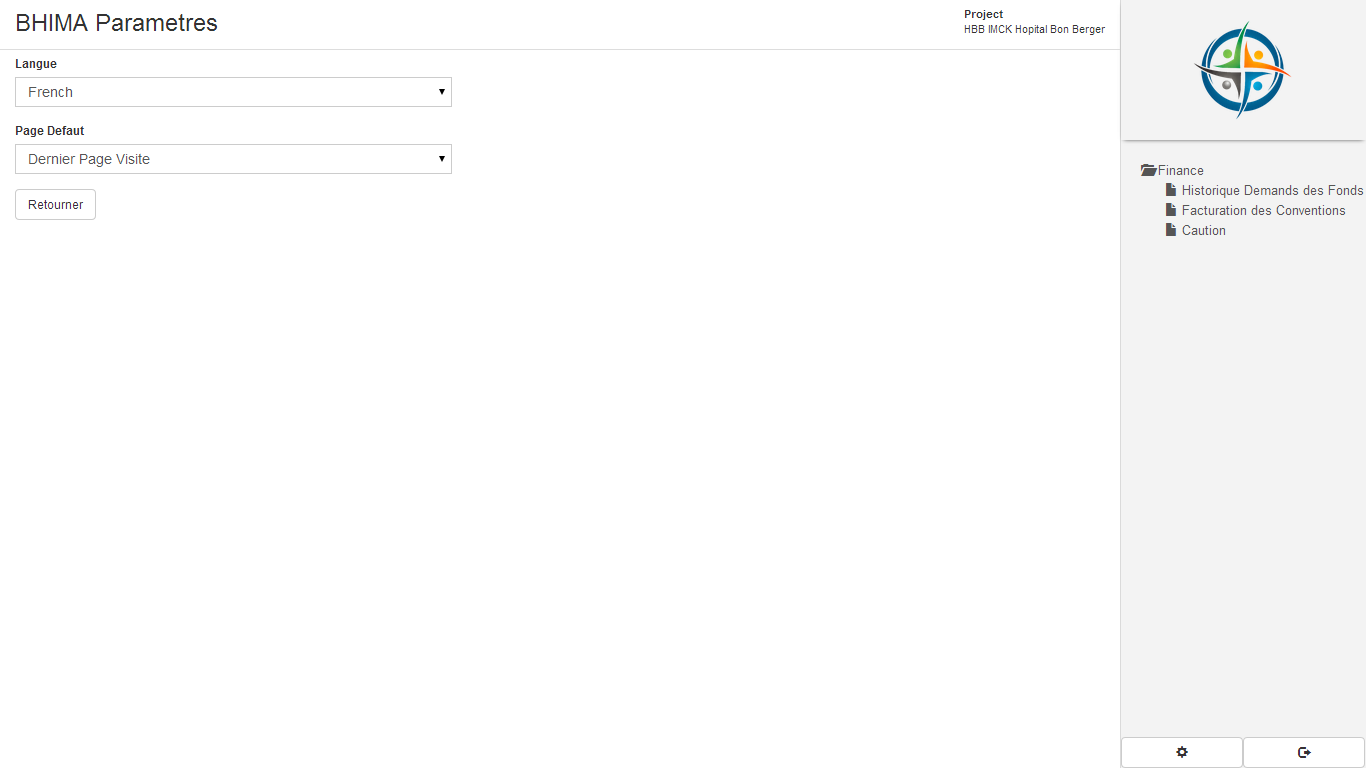
\includegraphics[width=10cm]{pic/changeLang.png}
\end{center}
\caption{Interface principale pour le changement de langue}
\label{Interface principale pour le changement de langue}
\end{figure} 

\section{Utilisation de l'arborescence de navigation}
L'arborescence de navigation contient les liens de chague module de l'application. Les modules sont regroupés en fonction de de leurs fonctionalités dans des dossiers tels que le dossier "Admin" affiché ci-dessous. Dans la première image, le dossier est fermé, en occultant tous les sous modules de ce module. Après le dossier est cliqué, une image d'un dossier ouvert montre que les contenus sont accessibles.

\begin{figure}[h]
\begin{center}
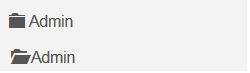
\includegraphics[width=4.5cm]{pic/folder_open_closed.png}
\end{center}
\caption{Etat d'un module ouvert et fermé}
\label{Etat d'un module ouvert et fermé}
\end{figure} 

Cliquant sur le dossier permet d'afficher la liste de sous modules sélectionné par l'utilisateur. Par exemple, ci-dessous, le dossier "Admin" est cliqué dans la premier illustration dans la séconde est ouverte tous ses sous modules.

\begin{figure}[h]
\begin{center}
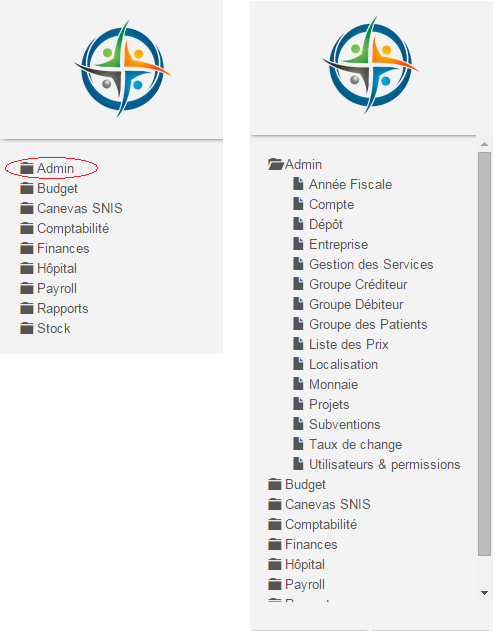
\includegraphics[width=8cm]{pic/open_folder.png}
\end{center}
\caption{Clique sur le dossier "admin" afin de pouvoir visualiser ses sous modules}
\label{Clique sur le dossier "admin" afin de pouvoir visualiser ses sous modules}
\end{figure} 


\newpage
\section{Les modules du système BHIMA}
Le système d'information BHIMA possède plusieurs modules qui sont représenté par l'arborescence ci-dessous.
\begin{figure}[h]
\begin{center}
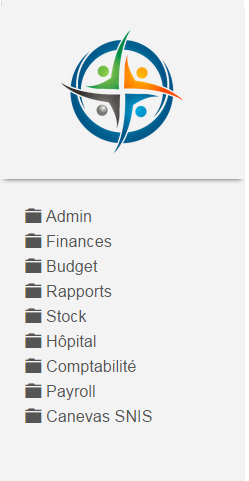
\includegraphics[width=4.5cm]{pic/arbo.png}
\end{center}
\caption{Arborescence du système}
\label{Arborescence du système}
Voici les différentes rubriques qui existent dans le système:
\end{figure} 
% Liste des modules
\begin{itemize}
\item Admin. %•
\item Budget
\item Canevas SNIS
\item Comptabilité
\item Finances
\item Hôpital
\item Payroll
\item Rapports
\item Stock
\end{itemize}


\newpage
%%%%%%%%%%%%%%%%%%%%%%%%%%%%%%%%%%%%%%%%%%%%%
%   MODULES DU SYSTEMES                     %
%%%%%%%%%%%%%%%%%%%%%%%%%%%%%%%%%%%%%%%%%%%%%
    
\chapter{Le module Admin}        
%////////////////////////////////////////////////%
% MODULE ADMIN
Le module admin est composé des sous modules qui permettent d'administrer le système. La figure ci-dessous représente avec exactitude ce module avec ses différents sous éléments.
\begin{figure}[h]
\begin{center}
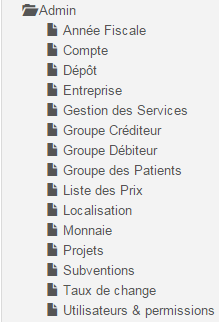
\includegraphics[width=4cm]{pic/s_admin.png}
\end{center}
\caption{Le module Admin et ses sous modules}
\label{Le module Admin et ses sous menus}
\end{figure} 

\newpage
\section{Taux d'échange}
Le module de taux de change, donne la possibilité de définir le taux d'échange du jour. Par souci d'intégrité des données, Le taux d'échange doit être défini chaque jour.


\begin{figure}[h]
\begin{center}
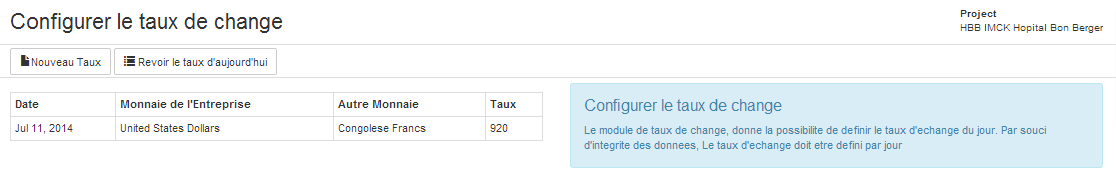
\includegraphics[width=16cm]{pic/FormulaireConfigRate.png}
\end{center}
\caption{Formulaire permettant de configurer le taux de change}
\label{Formulaire permettant de configurer le taux de change}
\end{figure}

\subsection{Nouveau Taux}
Lorsque l'utilisateur click sur le bouton 
\includegraphics[scale=0.7]{pic/NouveauTaux.png}
 Le formulaire ci-après apparait.

\begin{figure}[h]
\begin{center}
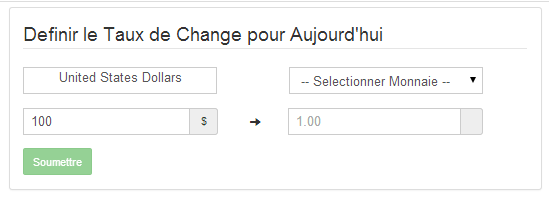
\includegraphics[width=12cm]{pic/DefinirTaux.png}
\end{center}
\caption{Formulaire permettant de definir le taux}
\label{Formulaire permettant de definir le taux}
\end{figure}
\begin{itemize}
\item \textbf{United States Dollars}: est la monnaie principale de l'application, l'équivalence avec d'autres monnaies ne doit se faire qu'avec la somme de 100 Dollars,
\item \textbf{Sélectionner Monnaie}: Affiche la liste des monnaies qui existe dans le système et la zone de saisie qui se retrouve en bas permet de préciser l'équivalence avec la monnaie principale.
\end{itemize}
Après avoir renseigné ce deux champs, un clique sur le bouton \textbf{Soumettre} permet de définir les taux du jour.

\newpage
\subsection{Revoir le taux d'aujourd'hui}
Un clic sur le bouton 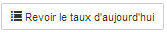
\includegraphics[scale=0.7]{pic/RevoirTaux.png} permet d'afficher toutes les informations sur le taux du jour, comme la montre la figure ci-dessous.
\begin{figure}[h]
\begin{center}
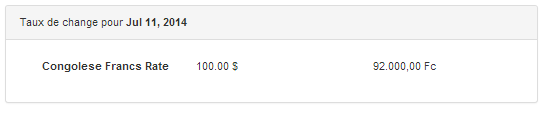
\includegraphics[width=12cm]{pic/ShowRate.png}
\end{center}
\caption{Aperçue du taux du jour}
\label{Aperçue du taux du jour}
\end{figure}
\newpage
\section{Localisation}
Gestions Emplacement permet d'enregistrer toutes les localisations possible pour l'enregistrement des patients. L'interface principale se présente comme de la manière suivante.

\begin{figure}[h]
\begin{center}
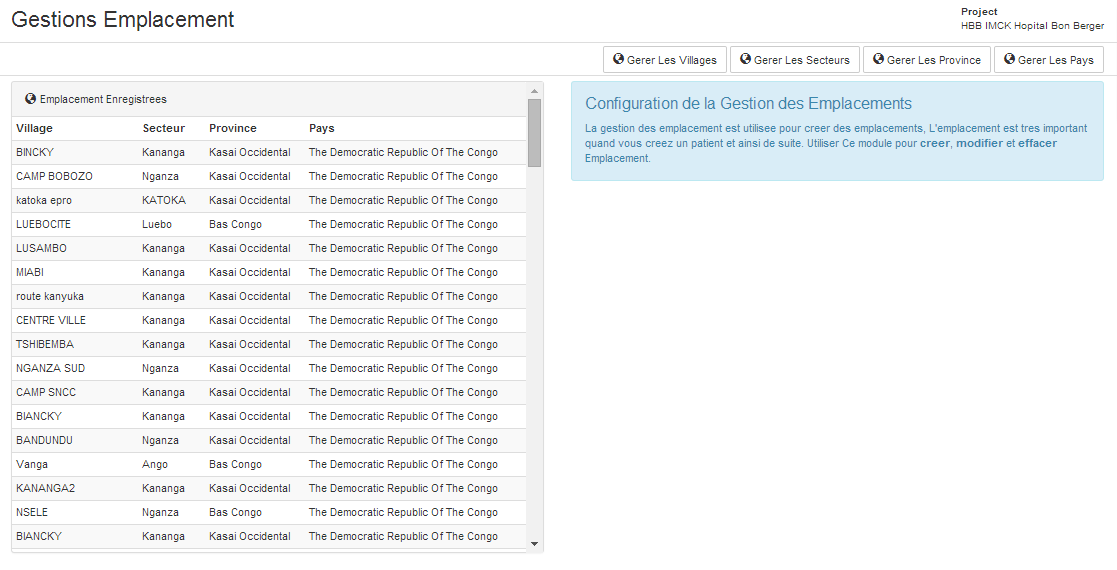
\includegraphics[width=14cm]{pic/AdminLocalisation.png}
\end{center}
\caption{Interface principale du module gestion des emplacement}
\label{Interface principale du module gestion des emplacement}
\end{figure}

Dans la partie droite l'on trouve le bouton qui permet d'ajouter les différents niveaux d'emplacement en commençant par la gestion des villages, des secteurs, des provinces ainsi que celui des pays. En dessous de ce menu de configuration est affiché sur un tableau les différents emplacements qui ont étaient enregistrés dans ce système. 
\newpage
\subsection{Gestion des villages}
Pour faire l'administration des villages, il suffit de cliquer sur le bouton\\ 
\includegraphics[scale=0.7]{pic/GererVillage.png}, ceci redirige vers la page qui permet une telle administration.

\begin{figure}[h]
\begin{center}
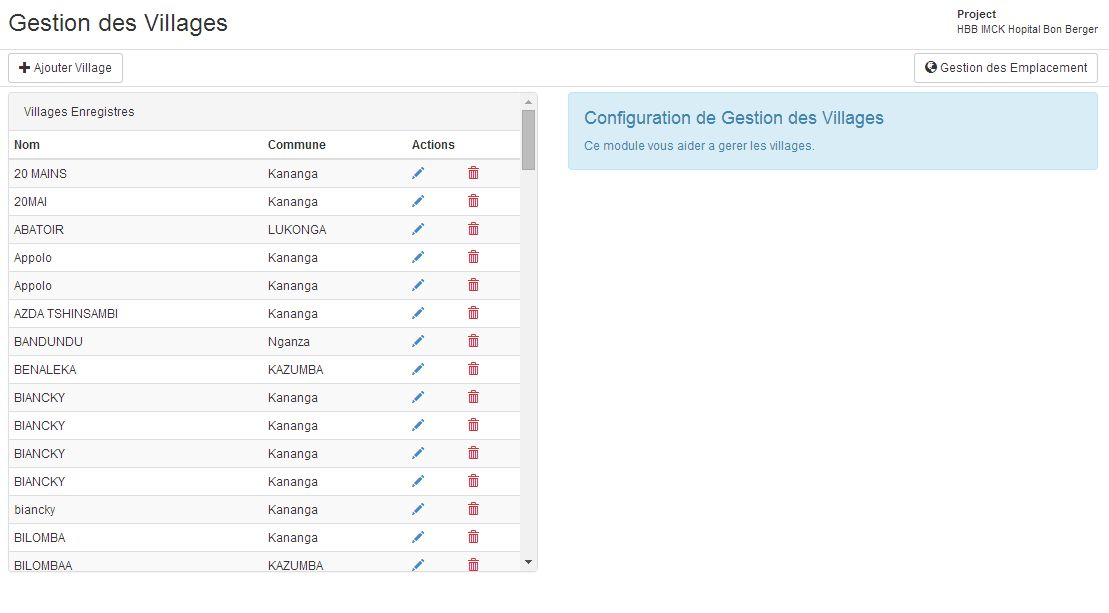
\includegraphics[width=14cm]{pic/AdminVillage.png}
\end{center}
\caption{Interface principale permettant d'administrer les villages}
\label{Interface principale permettant d'administrer les villages}
\end{figure}

Le bouton 
\includegraphics[scale=0.7]{pic/GestionEmplacement.png} redirige vers la page principale de la gestion des emplacements.

Le bouton 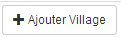
\includegraphics[scale=0.7]{pic/AddVillage.png} permet d'ajouter un village dans ladite liste.

\begin{figure}[h]
\begin{center}
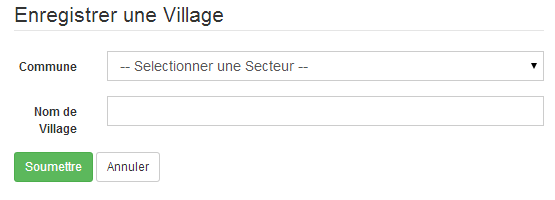
\includegraphics[width=14cm]{pic/FormAddVillage.png}
\end{center}
\caption{Formulaire permettant d'ajouter un village}
\label{Formulaire permettant d'ajouter un village}
\end{figure}

Le formulaire ci-haut apparait lorsqu'un utilisateur clique sur le bouton \textbf{ajouter village}. Ce formulaire possède deux champs, le premier \textbf{commune} renferme la liste de toutes les communes enregistré dans le système. 
L'enregistrement est effectif seulement si l'utilisateur clique sur le bouton soumettre. La liste des villages apparait sous forme de tableau. Ce tableau a trois rubriques. Le premier \textbf{Nom} renseigne sur le nom du village, le second \textbf{Commune} permet de savoir dans quelle commune se trouve le village et le dernier \textbf{Actions} renferme deux icônes le premier 
\includegraphics[scale=0.7]{pic/EditUser.png}  permet de modifier les informations sur un village et le second 
\includegraphics[scale=0.7]{pic/DeleteWRed.png}  permet de supprimer un village.

\subsection{Gérer les secteurs}
Pour faire l'administration des secteurs, il suffit de cliquer sur le bouton 
\includegraphics[scale=0.7]{pic/AdminSecteur.png} pour être redirigé vers la page qui permet une telle administration.

\begin{figure}[h]
\begin{center}
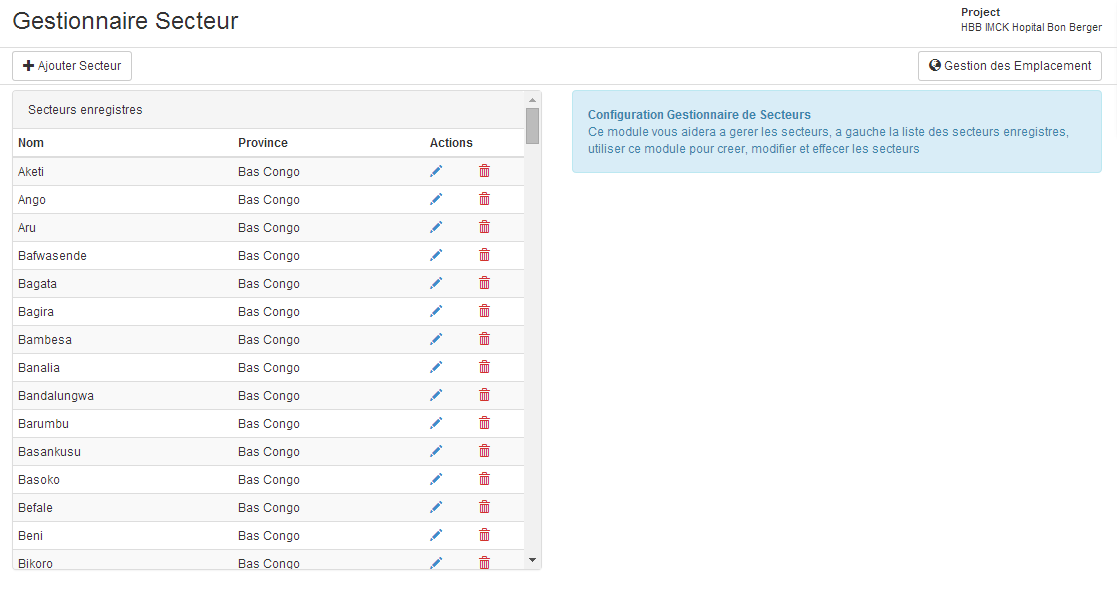
\includegraphics[width=12cm]{pic/FormulaireGestionSecteur.png}
\end{center}
\caption{Aperçue de l'interface permettant la gestion des secteurs}
\label{Aperçue de l'interface permettant la gestion des secteurs}
\end{figure}

Le bouton 
\includegraphics[scale=0.7]{pic/GestionEmplacement.png} redirige vers la page principale de la gestion des emplacements.
Le bouton 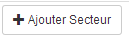
\includegraphics[scale=0.7]{pic/AddSecteur.png} permet d'ajouter un secteur dans ladite liste.

\begin{figure}[h]
\begin{center}
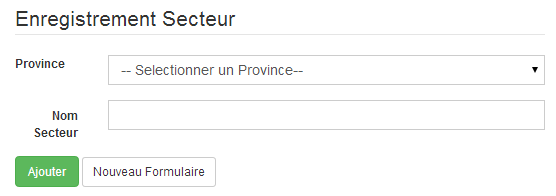
\includegraphics[width=10cm]{pic/FormAddSecteur.png}
\end{center}
\caption{Formulaire permettant d'ajouter les secteurs}
\label{Formulaire permettant d'ajouter les secteurs}
\end{figure}

Le formulaire ci-haut apparait lorsqu'un utilisateur clique sur le bouton \textbf{ajouter secteur}. Ce formulaire possède deux champs, le premier \textbf{Province} renferme la liste de toutes les provinces enregistré dans le système. 
L'enregistrement est effectif seulement si l'utilisateur clique sur le bouton Ajouter. La liste des secteurs apparait sous forme de tableau. Ce tableau a trois rubriques. Le premier\textbf{ Nom} renseigne sur le nom du secteur, le second \textbf{Province} permet de savoir dans quelle commune se trouve le village et le dernier \textbf{Actions} renferme deux icônes le premier 

\includegraphics[scale=0.7]{pic/EditUser.png}  permet de modifier les informations sur un secteur et le second 
 
\includegraphics[scale=0.7]{pic/DeleteWRed.png}  permet de supprimer un secteur.
\subsection{Gérer les provinces}
Pour faire l'administration des provinces, il suffit de cliquer sur le bouton 
\includegraphics[scale=0.7]{pic/AdminProvince.png} pour être redigé vers la page qui permet une telle administration.
\begin{figure}[h]
\begin{center}
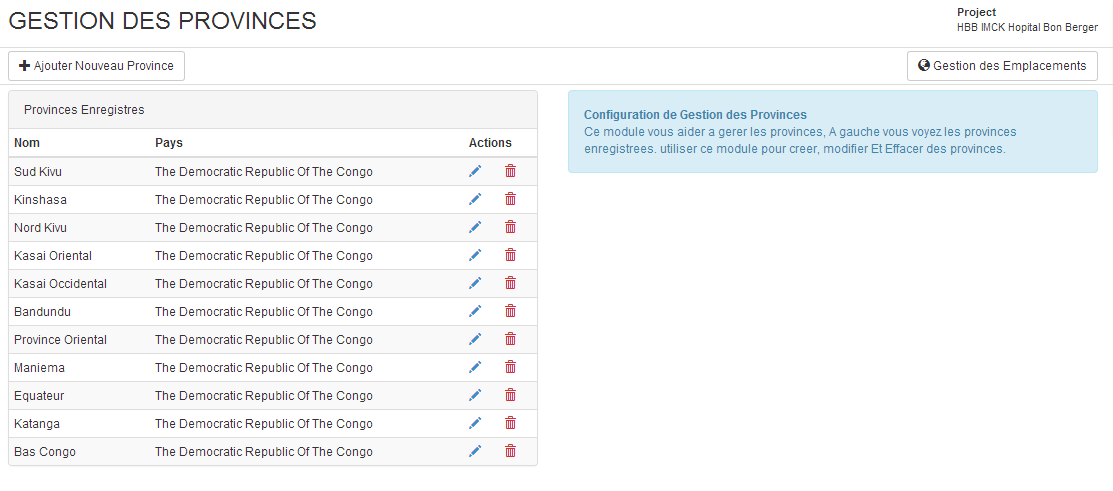
\includegraphics[width=14cm]{pic/InterfaceGestionProvince.png}
\end{center}
\caption{Interface principale permettant la gestion des provinces}
\label{Interface principale permettant la gestion des provinces}
\end{figure}

Le bouton 
\includegraphics[scale=0.7]{pic/GestionEmplacement.png} redirige vers la page principale de la gestion des emplacements.

Le bouton 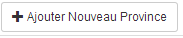
\includegraphics[scale=0.7]{pic/AddNewProvince.png} permet d'ajouter une province dans ladite liste.
\begin{figure}[h]
\begin{center}
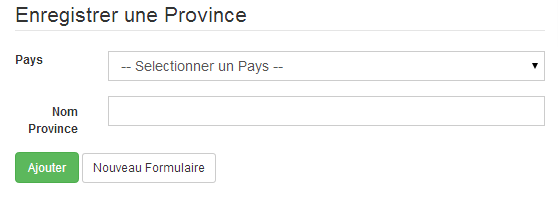
\includegraphics[width=10cm]{pic/FormNewProvince.png}
\end{center}
\caption{Formulaire permettant d'ajouter une province}
\label{Formulaire permettant d'ajouter une province}
\end{figure}


Le formulaire ci-haut apparait lorsqu'un utilisateur clique sur le bouton ajouter province. Ce formulaire possède deux champs, le premier Pays renferme la liste de tous les pays. 
L'enregistrement est effectif seulement si l'utilisateur clique sur le bouton Ajouter. La liste des provinces apparait sous forme de tableau. Ce tableau a trois rubriques. Le premier \textbf{Nom} renseigne sur le nom de la province, le second \textbf{Pays} permet de savoir dans quelle pays se trouve une province et le dernier \textbf{Actions} renferme deux icônes le premier 

\includegraphics[scale=0.7]{pic/EditUser.png}  permet de modifier les informations sur une province et le second  
\includegraphics[scale=0.7]{pic/DeleteWRed.png}  permet de supprimer une province.
\subsection{Gérer les pays}
Pour faire l'administration des pays, il suffit de cliquer sur le bouton 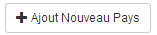
\includegraphics[scale=0.7]{pic/AddNewCountry.png}, ceci redirige vers la page qui permet une telle administration.
\begin{figure}[h]
\begin{center}
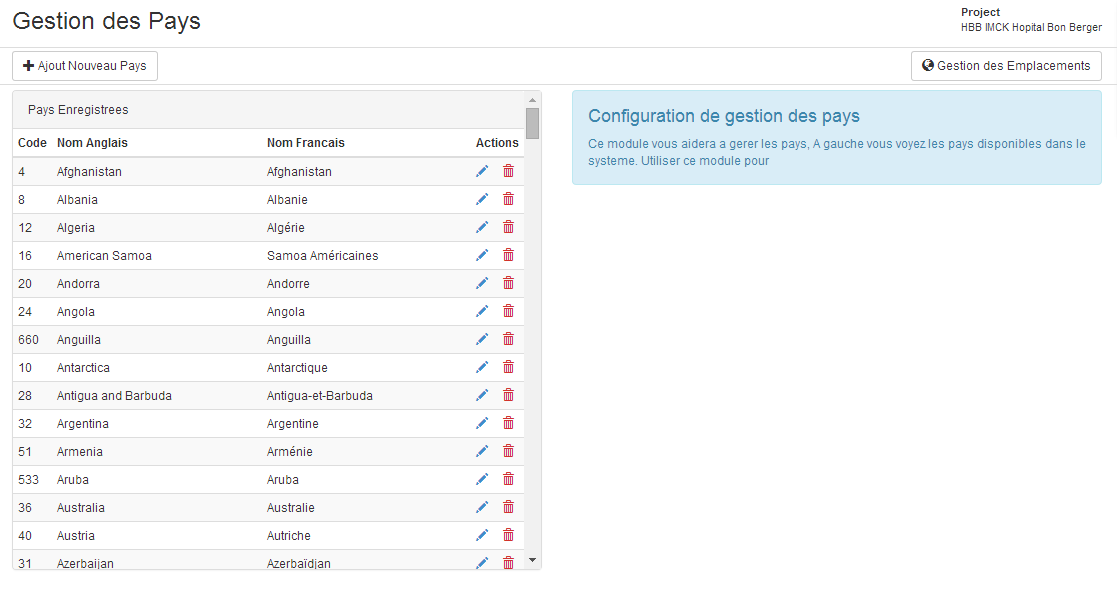
\includegraphics[width=14cm]{pic/AdminCountry.png}
\end{center}
\caption{Interface principale permettant la gestion des pays}
\label{Interface principale permettant la gestion des pays}
\end{figure}

Le bouton 
\includegraphics[scale=0.7]{pic/GestionEmplacement.png}  permet redirige vers la page principale de la gestion des emplacements.

Le bouton 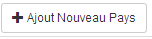
\includegraphics[scale=0.7]{pic/AddCountry.png} permet d'ajouter un pays dans ladite liste.

\begin{figure}[h]
\begin{center}
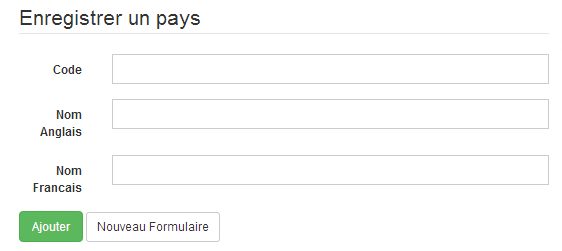
\includegraphics[width=10cm]{pic/SaveCountry.png}
\end{center}
\caption{Enregistrer un pays}
\label{Enregistrer un pays}
\end{figure}

Le formulaire ci-haut apparait lorsqu'un utilisateur clique sur le bouton \textbf{ajouter Nouveau pays}. Ce formulaire possède trois champs, le premier \textbf{Code} permet de donner un code à un pays ensuite un champ pour donner le nom du pays en \textbf{Anglais} et l'autre pour le \textbf{Français}.
L'enregistrement est effectif seulement si l'utilisateur clique sur le bouton Ajouter. La liste des pays apparait sous forme de tableau. Ce tableau a trois rubriques. Le premier \textbf{Code} renseigne sur le code qui a été attribué au pays, le second \textbf{Nom en anglais} suivi de \textbf{Nom}  et le dernier \textbf{Actions} renferme deux icônes le premier 
\includegraphics[scale=0.7]{pic/EditUser.png}  permet de modifier les informations sur un pays et le second 
\includegraphics[scale=0.7]{pic/DeleteWRed.png}  permet de supprimer un pays.

\newpage
\chapter{Le module finance}        
%////////////////////////////////////////////////%
Le module finance est composé des sous modules qui permettent d'administrer le finance. La figure ci-dessous représente avec exactitude ce module avec ses différents sous éléments.

\begin{figure}[h]
\begin{center}
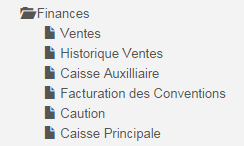
\includegraphics[width=6cm]{pic/FinanceArbo.png}
\end{center}
\caption{Arborescence du module Finance}
\label{Arborescence du module Finance}
\end{figure}


\section{Vente}
Le module de la vente permet de faire la facturation des produits et services à un patient. Son interface d'utilisation est simple et se présente de cette façon.

\begin{figure}[h]
\begin{center}
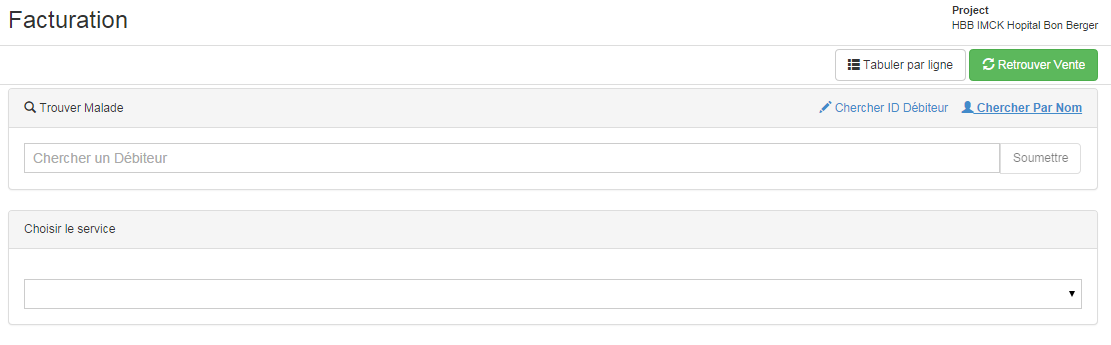
\includegraphics[width=14cm]{pic/InterfacePrinciFact.png}
\end{center}
\caption{Interface principale de la facturation}
\label{Interface principale de la facturation}
\end{figure}

Il y'a dans le coin droit deux boutons le premier 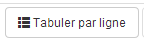
\includegraphics[scale=0.7]{pic/tabulerParLigne.png}  qui par défaut s'intitule comme ceci et comme son nom l'indique il permet de faire une tabulation par ligne mais si l'on clique sur ce bouton son intitulé change et ce bouton devient 
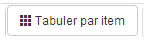
\includegraphics[scale=0.7]{pic/tabulerParItem.png}  qui change la propriété de la tabulation qui ne s'effectue plus par ligne mais par item. 

Le deuxième bouton 
\includegraphics[scale=0.7]{pic/RetrouverVente.png}  permet de retrouver une vente dont l'enregistrement a été interrompu pour une raison ou une autre. Par défaut ce bouton n'est pas cliquable, mais il le devient seulement si une opération de facturation n'est pas arrivée à terme et se présente comme ceci 
\includegraphics[scale=0.7]{pic/RetrouverVenteGreen.png}.

En dessous de cette zone réservé au bouton, il y'a une zone qui permet de rechercher un patient, le système propose deux façon de chercher un patient soit par son nom\textbf{ ID Débiteur} ou bien par son \textbf{Nom} 

\begin{figure}[h]
\begin{center}
\includegraphics[width=14cm]{pic/foundPatient.png}
\end{center}
\caption{Aperçue de la zone permettant de rechercher un patient}
\label{Aperçue de la zone permettant de rechercher un patient}
\end{figure}

Il existe une aussi une zone qui permet de spécifier le type de vente à opérer, il peut s'agir d'une vente distribuable ou bien d'une vente non distribuable. Une vente est dite distribuable si le patient pourrai aller se servir en produits pharmaceutiques et non distribuable si le patient à déjà consommer les dites produits. Par défaut c'est l'option \textbf{Distribuable} qui est coché par défaut.  

\begin{figure}[h]
\begin{center}
\includegraphics[width=14cm]{pic/TypeVente.png}
\end{center}
\caption{Aperçue de la zone permettant de spécifier le type de vente}
\label{Aperçue de la zone permettant de spécifier le type de vente}
\end{figure}

Après avoir lancer la recherche, les patients apparaissent sous forme d'une liste, une fois qu'on a retrouvé celui dont on a besoin, on le sélectionne et on clique sur le bouton soumettre, après cette étape il faudrait preciser dans quelle service est pris en charge le patient.

\begin{figure}[h]
\begin{center}
\includegraphics[width=14cm]{pic/PatientTrouver.png}
\end{center}
\caption{Aperçue du résultats de la recherche d'un patient}
\label{Aperçue du résultats de la recherche d'un patient}
\end{figure}

\newpage
Après avoir préciser le service, la figure ci-après représente l'interface principale permettant la facturation.

\begin{figure}[h]
\begin{center}
\includegraphics[width=14cm]{pic/FacturationInterface.png}
\end{center}
\caption{Aperçue de l'interface principale de la facturation}
\label{Aperçue de l'interface principale de la facturation}
\end{figure}

Sur cette interface on retrouve l'identité du patient dans le premier tableau, sur le second tableau on retrouve à droite le bouton \includegraphics[scale=0.7]{pic/AjouterItem.png} qui permet d'ajouter un item lors de l'opération de facturation mais par défaut l'interface de facturation n'est réservée qu'à un seul item.

Pour rechercher un item, il suffit de saisir sur dans la zone représenté dans la figure 
\includegraphics[scale=0.7]{pic/RechercheItem.png} pour que le système lance un filtre par rapport aux items qui existe dans le système.

\begin{figure}[h]
\begin{center}
\includegraphics[width=10cm]{pic/AppRechercheItem.png}
\end{center}
\caption{Apperçue du formulaire de la recherche des Itèms}
\label{Apperçue du formulaire de la recherche des Itèms}
\end{figure}

Après avoir sélectionné un item, la zone de saisie se modifier et son prix unitaire apparait automatique, ce prix fait automatiquement référence à la liste de prix du groupe de malade dans lequel le patient appartient. 


\begin{figure}[h]
\begin{center}
\includegraphics[width=14cm]{pic/UpdateItem.png}
\end{center}
\caption{Formulaire permettant de preciser la quantité d'un Item}
\label{Formulaire permettant de preciser la quantité d'un Item}
\end{figure}


La quantité de l'item est à présent éditable, le système donne la possibilité d'ajouter autant d'item que possible simplement en cliquant sur le bouton 
\includegraphics[scale=0.7]{pic/PlusAddItem.png}.
 
Pour achever l'opération des facturations, il suffit de cliquer sur le bouton soumettre comme le monte la figure ci-après.

\begin{figure}[h]
\begin{center}
\includegraphics[width=14cm]{pic/InterfaceSoumettreFacture.png}
\end{center}
\caption{Aperçue du processus de la facturation}
\label{Aperçue du processus de la facturation}
\end{figure}

Cette action permet d'afficher une facture pour le patient, et grâce à cette facture le patient pourra aller payer à la caisse.


\begin{figure}[h]
\begin{center}
\includegraphics[width=14cm]{pic/InvoiceView.png}
\end{center}
\caption{Spécimen de facture produit par le système}
\label{Spécimen de facture produit par le système}
\end{figure}

\newpage

\section{Historique des ventes}
L'historique de vente permet de connaitre l'historique des toutes les opérations liée à la vente dans le système, son interface principale se présente de cette façon.


\begin{figure}[h]
\begin{center}
\includegraphics[width=14cm]{pic/HistoVente.png}
\end{center}
\caption{Interface principale du module Historique des ventes}
\label{Interface principale du module Historique des ventes}
\end{figure}

Les données qui se présente par défaut et celui du jour en cours mais il y'a la possibilité de le modifier soit en sélectionnant dans la liste de choix, un autre critère d'affichage, sur cette liste de choix comme le montre la figure ci-après, on a le choix \textbf{entre Aujourd'hui, Cette semaine et ce mois} 


\begin{figure}[h]
\begin{center}
\includegraphics[width=4cm]{pic/SelectJour.png}
\end{center}
\caption{Aperçue de l'option permettant de rechercher une période de vente}
\label{Aperçue de l'option permettant de rechercher une période de vente}
\end{figure}

Mais juste à côté de cette liste de choix, on a la possibilité de préciser une plage de valeur en précisant pour ce cas la date initiale et la date terminale.

\begin{figure}[h]
\begin{center}
\includegraphics[width=8cm]{pic/SelectPlageValeur.png}
\end{center}
\caption{Aperçue de l'option permettant de rechercher l'historique des ventes dans une plage de temps}
\label{Aperçue de l'option permettant de rechercher l'historique des ventes dans une plage de temps}
\end{figure}

Le tableau de l'historique de vente comporte 5 colonnes dont l'une pour la\textbf{ date} de de la vente, le second pour \textbf{ID }de la vente, le \textbf{nom du patient}, le \textbf{montant} de la vente ainsi qu'une dernière colonne consacrée à \textbf{l'actions}. Cette dernière permet comporte deux options \includegraphics[scale=0.7]{pic/FactureF.png}  et \includegraphics[scale=0.7]{pic/NoteCredit.png}, Le premier facture permet de visualiser  la facture qui concerne cette vente, le second note de crédit permet d'annuler une vente. 

Lorsqu'on clique sur \includegraphics[scale=0.7]{pic/NoteCredit.png}  l'interface ci-dessous apparait.

\begin{figure}[h]
\begin{center}
\includegraphics[width=14cm]{pic/NoteCreditMenu.png}
\end{center}
\caption{Interface permettant d'annuler une vente}
\label{Interface permettant d'annuler une vente}
\end{figure}

Pour voir le détaille de la facture il suffit de cliquer sur le bouton \includegraphics[scale=0.7]{pic/SeeInvoice.png} qui se trouve dans le coin droit de la zone Détaille de facture   


Et pour annuler une vente il suffit de cliquer sur le bouton \includegraphics[scale=0.7]{pic/SubmitNoteCredit.png}  pour que s'affiche sur l'écran l'interface ci-dessous.

\begin{figure}[h]
\begin{center}
\includegraphics[width=14cm]{pic/RecetteCredit.png}
\end{center}
\caption{Aperçue d'une vente qui a été annulée}
\label{Aperçue d'une vente qui a été annulée}
\end{figure}

Et quand on revient sur la page principale de l'historique de vente on peut se rendre compte que les ventes annulés se colorent différemment des autres, comme on peut le constaté dans la figure ci-dessous.

\begin{figure}[h]
\begin{center}
\includegraphics[width=14cm]{pic/HistoriqueVenteDell.png}
\end{center}
\caption{Aperçue de l'historique des ventes avec des ventes annulées}
\label{Aperçue de l'historique des ventes avec des ventes annulées}
\end{figure}

\newpage
\chapter{Le module Rapports}        
%////////////////////////////////////////////////%
Le module rapports permet de pouvoir visualiser plusieurs types des rapports résultants du fonctionnements du système, La figure ci-dessous représente avec exactitude ce module avec les différents sous éléments.

\begin{figure}[h]
\begin{center}
\includegraphics[width=4cm]{pic/ArboReport.png}
\end{center}
\caption{Arborescence du module Rapports}
\label{Arborescence du module Rapports}
\end{figure}

\newpage
\section{Rapport d'enregistrement des Patients}
Le rapport d'enregistrement des patients permet de visualiser l'historique d'enregistremet des patients dans le système. L'interface principale permettant de voire le rapport d'enregistrement des patients se présente de la manière suivante. 

\begin{figure}[h]
\begin{center}
\includegraphics[width=10cm]{pic/RapportEnrPatient.png}
\end{center}
\caption{Aperçue de l'interface principale du rapport d'enregistrement des patients}
\label{Aperçue de l'interface principale du rapport d'enregistrement des patients}
\end{figure}


La première zone permet de sélectionner le projet pour lequel on voudriai visualiser le rapport d'enregistrement, il y'a aussi une zone qui permet de spécifier l'écheance temporelle  ou bien spécifier directement la date du début et celle de la fin de la recherche. 

Le bouton générer permet l'affichage du tableau du rapport d'enregistrement des patients. L'interface permettant de visualier le rapport se présente de la manière suivante. Au dessus on retrouve deux boutons. le prémier 
\includegraphics[scale=0.7]{pic/Print.png} permet d'imprimer le rapport et le second \includegraphics[scale=0.7]{pic/refresh.png} permet de faire une nouvelle recherche.


\begin{figure}[h]
\begin{center}
\includegraphics[width=12cm]{pic/PatientSaving.png}
\end{center}
\caption{Aperçue du résultat du rapport d'enregistrement des patients}
\label{Aperçue du résultat du rapport d'enregistrement des patients}
\end{figure}


\newpage
\section{Rapport des patients}
Le rapport des patiens permet de visualiser l'état financier d'un patient. son interface principale se présente de la manière suivante. 

\begin{figure}[h]
\begin{center}
\includegraphics[width=10cm]{pic/EtatFInPat.png}
\end{center}
\caption{Aperçue de l'interface principale de l'état financier d'un patient}
\label{Aperçue de l'interface principale de l'état financier d'un patient}
\end{figure}

Le formulaire possède une zone qui permet la recherche d'un patient dans la liste des patients enregistrés, le bouton générer permet l'affichage du tableau du rapport des employés. L'interface permettant de visualier le rapport se présente de la manière suivante. Au dessus on retrouve deux boutons. le prémier 
\includegraphics[scale=0.7]{pic/Print.png} permet d'imprimer le rapport et le second \includegraphics[scale=0.7]{pic/refresh.png} permet de faire une nouvelle recherche.

Voici un apperçue de la situation financière d'un patient.

\begin{figure}[h]
\begin{center}
\includegraphics[width=14cm]{pic/RapEtFinPatient.png}
\end{center}
\caption{Aperçue du rapport financier d'un patient}
\label{Aperçue du rapport financier d'un patient}
\end{figure}



%////////////////////////////////////////////////%
\newpage
\chapter{Hôpital}        

Le module Hôpital est composé des sous modules qui permettent d'administrer les patients. La figure ci-dessous représente avec exactitude ce module avec ses différents sous éléments.

\begin{figure}[h]
\begin{center}
\includegraphics[width=6cm]{pic/HopitalArbo.png}
\end{center}
\caption{Arborescence du module Hôpital}
\label{Arborescence du module Hôpital}
\end{figure}

\section{Enregistrement des Patients}
Le module permttant l'enregistrement de patient permet d'enregistrer les patients dans le système, lors de toute opération d'enregistrement il est nécessaire de pouvoir spécifier dans quelle circonstance se derroule l'enregistrement, il peut s'agir d'un nouveau patient à l'hôpital, mais aussi des patients qui ont été enregistrés, et ont une histoire prescription / vente avec l'hôpital, mais n'ont jamais été enregistrée dans le système BHIMA et dans le dernier cas pour le patient qui existe déjà dans le système. 

Le formulaire permettant l'enregistrement des patients dans le système est subdivisé en quatres parties, la prémière partie se présente de la manière suivante.

\begin{figure}[h]
\begin{center}
\includegraphics[width=12cm]{pic/DetailPatient.png}
\end{center}
\caption{Aperçue de la partie Détail Patient}
\label{Aperçue de la partie Détail Patient}
\end{figure}

Dans cette prémière partie il est nécessaire de fournir les informations liés au Prénom ainsi que le nom du patient, sa date de naissance ainsi que le sexe du patient.

La seconde partie est reservée à l'emplacement du patient, pour cela il est nécessaire de pouvoir renseigner l'emplacement origin mais aussi l'emplacement dans la quelle se trouve présentement le patient, voici un apperçue du module qui permet de sélectionner l'emplacement origine et présent d'un patient.

\begin{figure}[h]
\begin{center}
\includegraphics[width=12cm]{pic/EmplacementPatient.png}
\end{center}
\caption{Aperçue de l'interface liée à l'emplacement d'un patient}
\label{Aperçue de l'interface liée à l'emplacement d'un patient}
\end{figure}

Il est nécessaire de pouvoir fournir les informations liées au pays du patient, sa province, son secteur, ainsi que son village d'origine en plus de cela il faudrait aussi preciser l'emplacement présent du patient.
\newpage
La troisième partie consacré à la finance permet d'attribué un groupe débiteur à un patient, pour le patient qui n'appartienne pas à une convention sont généralement enregistrés comme étant des patients payants cash. mais si non il faudrait les attribuer à des bons groupes débiteurs. Voici l'apperçue du formulaire permettant l'attribution des patients à des groupes débiteurs.

\begin{figure}[h]
\begin{center}
\includegraphics[width=7cm]{pic/SelectGrDebiteur.png}
\end{center}
\caption{Aperçue de l'interface permettant la sélection d'un groupe débiteur}
\label{Aperçue de l'interface permettant la sélection d'un groupe débiteur}
\end{figure} 
 
La quatrième partie permet concerne les informations optionnelles, liés à un patient il s'agit du numéro de téléphone, l'adresse e-mail, la rue, le nom du pére, de la mère, la religion, Etat civil, la profession, etc...
Voici l'apperçue du formulaire qui permet de permet de renseigner ses informations optionnelles.

\begin{figure}[h]
\begin{center}
\includegraphics[width=8cm]{pic/InfoOptionnel.png}
\end{center}
\caption{Aperçue de l'interface permettant l'engistrement des informations optionnelles}
\label{Aperçue de l'interface permettant l'engistrement des informations optionnelles}
\end{figure} 
Dans la partie droite du formulaire on la zone permettant de preciser le type d'enregistrement, à l'exception des deux premières options la troisième permet de rechercher les informations liées aux patients. voici comment se présente l'interface permettant de préciser le type d'enregistrement à appliquer lors de l'enregistrement d'un patient. 

Et une fois qu'on a choisi l'option d'enregistrement, il suffit de cliquer sur le bouton \includegraphics[scale=0.7]{pic/EnregPatient.png} pour rendre effective l'enregistrement du patient dans le système.

\begin{figure}[h]
\begin{center}
\includegraphics[width=8cm]{pic/TypeEnregistrement.png}
\end{center}
\caption{Aperçue de l'interface permettant de préciser le type d'enregistrement}
\label{Aperçue de l'interface permettant de préciser le type d'enregistrement}
\end{figure}  
\newpage
Lorsqu'on coche sur la dernière option, l'interface d'enregistrement change d'apparence et la zone permettant de rechercher un patient apparait avec la possibilité de rechercher un patient soit par le \textbf{ID débiteur} ou bien par \textbf{le nom du malade}. La figure ci-dessous illustre la recherche d'un patient déjà enregistré dans le système.

\begin{figure}[h]
\begin{center}
\includegraphics[width=8cm]{pic/ApRecherche.png}
\end{center}
\caption{Aperçue de l'interface permettant la recherche d'un patient déjà enregistré}
\label{Aperçue de l'interface permettant la recherche d'un patient déjà enregistré}
\end{figure}  

Et si l'on clique sur le bouton \textbf{Soumettre pour que s'affiche les informations liées au patient}

\newpage
\section{Recherche des patients}
Le module recherche des patients, permet de faire des recherches détaillées par rapport aux informations liées à des patients, le système permet de pouvoir faire la recherche en se basant soit par le nom, le prénom, l'année de naissance ainsi que le sexe.

\begin{figure}[h]
\begin{center}
\includegraphics[width=11cm]{pic/recherchePatient.png}
\end{center}
\caption{Aperçue de l'interface permettant la recherche détaillées des patients}
\label{Aperçue de l'interface permettant la recherche détaillées des patients}
\end{figure}  

Pour pouvoir lancer la recherche il suffit de cliquer sur le bouton \includegraphics[scale=0.7]{pic/ExeButton.png}

Il est possible de pouvoir rechercher les patients en incluant la localisation géographique des patients dans la recherche grâce au bouton \includegraphics[scale=0.7]{pic/LocalisationRecherche.png}

\subsection{Illustration de la recheche détaillée}
Supposons qu'on a besoin de rechercher les femmes qui sont nées en 1960. il suffirait de remplir la fiche de la manière suivante, et appuiyer sur le bouton Exécuter pour que s'affiche en dessous du formulaire les résultats de la recherche. 

\begin{figure}[h]
\begin{center}
\includegraphics[width=11cm]{pic/RechecheDetailler.png}
\end{center}
\caption{Aperçue de l'interface permettant de visualiser les résultats de la recherche}
\label{Aperçue de l'interface permettant de visualiser les résultats de la recherche}
\end{figure} 

\subsection{Illustration de la recheche détaillée incluant la localisation géographique}
Supposont cette fois ci qu'on aimerai connaitre combien y a t'il des femmes qui sont né en 1992 et qui habitent dans le village de TSHIKAJI.

\begin{figure}[h]
\begin{center}
\includegraphics[width=11cm]{pic/RechercheDetGeo.png}
\end{center}
\caption{Aperçue d'une recherche incluant la localisation géographique}
\label{Aperçue d'une recherche incluant la localisation géographique}
\end{figure} 
 
\newpage
\section{Assignations groupes débiteurs}
Permet d'assigné un patient dans des groupes débiteurs qui bénéficie des certaines avantages pendant le processus de la vente et de la facturation des malades.

Pour assigner un patient à un groupe, il faudrait prémièrement le rechercher et en suite cocher dans les différentes assignations qu'il lui faut en suite clique sur le bouton \textbf{Sauver changement}

Voici comment se compose l'interface principale de ce module.

\begin{figure}[h]
\begin{center}
\includegraphics[width=11cm]{pic/AssPatients.png}
\end{center}
\caption{Aperçue de l'interface permettant de rechercher un patient}
\label{Aperçue de l'interface permettant de rechercher un patient}
\end{figure} 

Après avoir rechercher un patient, il suffit juste de cliquer sur le bouton soumettre pour qu'apparaise l'interface permettant de chocher les différents assignations nécessaire.

\begin{figure}[h]
\begin{center}
\includegraphics[width=11cm]{pic/AssiGames.png}
\end{center}
\caption{Aperçue de l'interface permettant l'assignations à des groupes des patients}
\label{Aperçue de l'interface permettant l'assignations à des groupes des patients}
\end{figure} 

Si l'on a choisi un patient mais qu'on aimerai choisir un autre il suffit de cliquer sur le bouton \includegraphics[scale=0.7]{pic/ComeBack.png}  pour revenir à l'interface permettant de rechercher un patient.

Si l'on veut aussi modifier l'assignation d'un patient à un groupe, il suffit de suivre le même procedure que pour l'assignation mais dans ce cas, les groupes dans lesquelles a été assigné le patient seront coché en avance, une fois que les groupes ont été modifier, il suffit à nouveau de cliquer sur le bouton \includegraphics[scale=0.7]{pic/SaveChang.png} pour pouvoir enregistrer les changements.

\section{Changer groupe débiteur}
Le module changer le groupe débiteur est en fait un module permettant l'affectation des patients à des groupes débiteurs, le processus d'affection des patients à des groupes débiteurs consiste premièrement à rechercher le patient et en suite à trouver dans quelle groupe le placer.

Voici l'interface principale permettant l'affectation des patients à des groupes débiteurs.

\begin{figure}[h]
\begin{center}
\includegraphics[width=11cm]{pic/AffeGrDeb.png}
\end{center}
\caption{Aperçue de l'interface permettant l'affectation d'un patient à un groupe créditeur}
\label{Aperçue de l'interface permettant l'affectation d'un patient à un groupe créditeur}
\end{figure}

\newpage
Une fois qu'un débiteur a été trouver, l'interface d'utilisation change et dans sa prémière partie, fourni les informations liées à un patient et dans la séconde partie apparait la liste des groupes débiteurs existant au sein dans le système, et si le patient appartient déjà à un groupe débiteur ce dernier sera directement sélectionner par défaut.

Si le choix du groupe débiteur est fait, il suffit maintenant de cliquer sur le bouton \textbf{Soumettre} pour pouvoir confirmer l'affection d'un patient à un groupe débiteur, ce module est utilisé dans la plupart des temps si l'on veut modifier le groupe débiteur dans lequel appartient un patient.

\begin{figure}[h]
\begin{center}
\includegraphics[width=11cm]{pic/AffectGrDebiteur.png}
\end{center}
\caption{Aperçue du processus d'affectation}
\label{Aperçue du processus d'affectation}
\end{figure}


%%%%%%%%%%%%%%%%%%%%%%%%%%%%%%%%%%%%%%%%%%%%%%%%%
% Table des matieres
\tableofcontents
\end{document}